\documentclass[twoside]{book}

% Packages required by doxygen
\usepackage{fixltx2e}
\usepackage{calc}
\usepackage{doxygen}
\usepackage[export]{adjustbox} % also loads graphicx
\usepackage{graphicx}
\usepackage[utf8]{inputenc}
\usepackage{makeidx}
\usepackage{multicol}
\usepackage{multirow}
\PassOptionsToPackage{warn}{textcomp}
\usepackage{textcomp}
\usepackage[nointegrals]{wasysym}
\usepackage[table]{xcolor}

% Font selection
\usepackage[T1]{fontenc}
\usepackage[scaled=.90]{helvet}
\usepackage{courier}
\usepackage{amssymb}
\usepackage{sectsty}
\renewcommand{\familydefault}{\sfdefault}
\allsectionsfont{%
  \fontseries{bc}\selectfont%
  \color{darkgray}%
}
\renewcommand{\DoxyLabelFont}{%
  \fontseries{bc}\selectfont%
  \color{darkgray}%
}
\newcommand{\+}{\discretionary{\mbox{\scriptsize$\hookleftarrow$}}{}{}}

% Page & text layout
\usepackage{geometry}
\geometry{%
  a4paper,%
  top=2.5cm,%
  bottom=2.5cm,%
  left=2.5cm,%
  right=2.5cm%
}
\tolerance=750
\hfuzz=15pt
\hbadness=750
\setlength{\emergencystretch}{15pt}
\setlength{\parindent}{0cm}
\setlength{\parskip}{3ex plus 2ex minus 2ex}
\makeatletter
\renewcommand{\paragraph}{%
  \@startsection{paragraph}{4}{0ex}{-1.0ex}{1.0ex}{%
    \normalfont\normalsize\bfseries\SS@parafont%
  }%
}
\renewcommand{\subparagraph}{%
  \@startsection{subparagraph}{5}{0ex}{-1.0ex}{1.0ex}{%
    \normalfont\normalsize\bfseries\SS@subparafont%
  }%
}
\makeatother

% Headers & footers
\usepackage{fancyhdr}
\pagestyle{fancyplain}
\fancyhead[LE]{\fancyplain{}{\bfseries\thepage}}
\fancyhead[CE]{\fancyplain{}{}}
\fancyhead[RE]{\fancyplain{}{\bfseries\leftmark}}
\fancyhead[LO]{\fancyplain{}{\bfseries\rightmark}}
\fancyhead[CO]{\fancyplain{}{}}
\fancyhead[RO]{\fancyplain{}{\bfseries\thepage}}
\fancyfoot[LE]{\fancyplain{}{}}
\fancyfoot[CE]{\fancyplain{}{}}
\fancyfoot[RE]{\fancyplain{}{\bfseries\scriptsize Generated by Doxygen }}
\fancyfoot[LO]{\fancyplain{}{\bfseries\scriptsize Generated by Doxygen }}
\fancyfoot[CO]{\fancyplain{}{}}
\fancyfoot[RO]{\fancyplain{}{}}
\renewcommand{\footrulewidth}{0.4pt}
\renewcommand{\chaptermark}[1]{%
  \markboth{#1}{}%
}
\renewcommand{\sectionmark}[1]{%
  \markright{\thesection\ #1}%
}

% Indices & bibliography
\usepackage{natbib}
\usepackage[titles]{tocloft}
\setcounter{tocdepth}{3}
\setcounter{secnumdepth}{5}
\makeindex

% Hyperlinks (required, but should be loaded last)
\usepackage{ifpdf}
\ifpdf
  \usepackage[pdftex,pagebackref=true]{hyperref}
\else
  \usepackage[ps2pdf,pagebackref=true]{hyperref}
\fi
\hypersetup{%
  colorlinks=true,%
  linkcolor=blue,%
  citecolor=blue,%
  unicode%
}

% Custom commands
\newcommand{\clearemptydoublepage}{%
  \newpage{\pagestyle{empty}\cleardoublepage}%
}

\usepackage{caption}
\captionsetup{labelsep=space,justification=centering,font={bf},singlelinecheck=off,skip=4pt,position=top}

%===== C O N T E N T S =====

\begin{document}

% Titlepage & ToC
\hypersetup{pageanchor=false,
             bookmarksnumbered=true,
             pdfencoding=unicode
            }
\pagenumbering{roman}
\begin{titlepage}
\vspace*{7cm}
\begin{center}%
{\Large My Project }\\
\vspace*{1cm}
{\large Generated by Doxygen 1.8.11}\\
\end{center}
\end{titlepage}
\clearemptydoublepage
\tableofcontents
\clearemptydoublepage
\pagenumbering{arabic}
\hypersetup{pageanchor=true}

%--- Begin generated contents ---
\chapter{File Index}
\section{File List}
Here is a list of all files with brief descriptions\+:\begin{DoxyCompactList}
\item\contentsline{section}{\hyperlink{Lab1_8c}{Lab1.\+c} }{\pageref{Lab1_8c}}{}
\end{DoxyCompactList}

\chapter{File Documentation}
\hypertarget{BrickGame_8cpp}{}\section{Brick\+Game.\+cpp File Reference}
\label{BrickGame_8cpp}\index{Brick\+Game.\+cpp@{Brick\+Game.\+cpp}}
{\ttfamily \#include $<$iostream.\+h$>$}\\*
{\ttfamily \#include $<$conio.\+h$>$}\\*
{\ttfamily \#include $<$ctype.\+h$>$}\\*
{\ttfamily \#include $<$process.\+h$>$}\\*
{\ttfamily \#include $<$dos.\+h$>$}\\*
{\ttfamily \#include $<$stdlib.\+h$>$}\\*
{\ttfamily \#include $<$graphics.\+h$>$}\\*
{\ttfamily \#include $<$stdio.\+h$>$}\\*
Include dependency graph for Brick\+Game.\+cpp\+:
\nopagebreak
\begin{figure}[H]
\begin{center}
\leavevmode
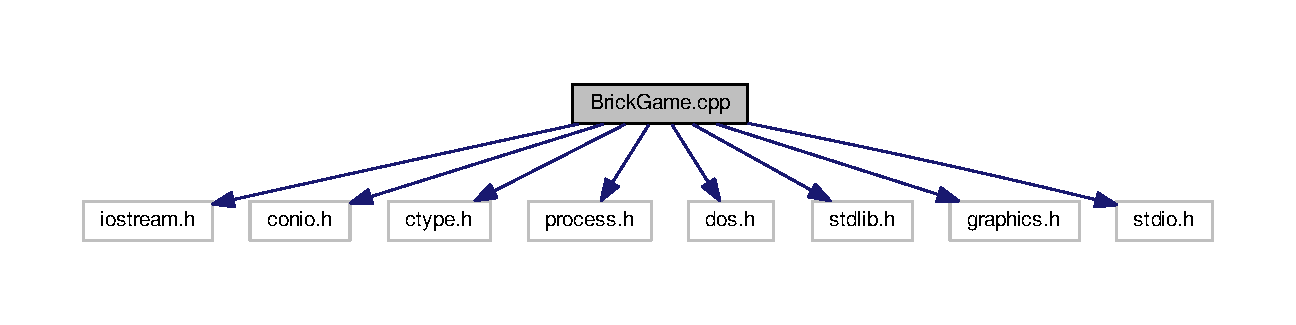
\includegraphics[width=350pt]{BrickGame_8cpp__incl}
\end{center}
\end{figure}
\subsection*{Macros}
\begin{DoxyCompactItemize}
\item 
\#define \hyperlink{BrickGame_8cpp_a070d2ce7b6bb7e5c05602aa8c308d0c4}{N\+U\+LL}~0
\item 
\#define \hyperlink{BrickGame_8cpp_a7ebc9a785e5ab85457c98595aac81589}{Y\+ES}~1
\item 
\#define \hyperlink{BrickGame_8cpp_a996bde01ecac342918f0a2c4e7ce7bd5}{NO}~0
\item 
\#define \hyperlink{BrickGame_8cpp_a4af1b6159e447ba72652bb7fcdfa726e}{E\+SC}~0x1b			/$\ast$ Define the escape key	$\ast$/
\end{DoxyCompactItemize}
\subsection*{Functions}
\begin{DoxyCompactItemize}
\item 
void \hyperlink{BrickGame_8cpp_a7f34e789c6e833bd0e987f5f5cfca365}{Initialize} (void)
\item 
void \hyperlink{BrickGame_8cpp_a45be7d4887a46847a975e931a370d809}{Say\+Goodbye} (void)
\item 
void \hyperlink{BrickGame_8cpp_a0b371e2e9982e6b8df3fc8db277285ef}{changetextstyle} (int font, int direction, int charsize)
\item 
\hyperlink{BrickGame_8cpp_a52fea2da489477c962bf950eea007ba6}{mainscreen} ()
\item 
\hyperlink{BrickGame_8cpp_a1bdb5b7ff52377e69d4bd2db765f1a68}{screen} ()
\item 
and bulbs rounded form \hyperlink{BrickGame_8cpp_a184670f140c6f80bd53e65727abbeb32}{bricks} ()
\item 
\hyperlink{BrickGame_8cpp_a3f3f0c01c08db0ab9ca1a3abeb9d5fc4}{delbrick} (int, int)
\item 
\hyperlink{BrickGame_8cpp_ae3891f6a73dc70fd3d09697a9b25dea8}{bell} (int)
\end{DoxyCompactItemize}
\subsection*{Variables}
\begin{DoxyCompactItemize}
\item 
int \hyperlink{BrickGame_8cpp_a9884e5cf9382e9d9bb81413a9b679058}{MaxX}
\item 
int \hyperlink{BrickGame_8cpp_a7ba407ecaa7dceed55a8ab787d28049f}{MaxY}
\item 
int \hyperlink{BrickGame_8cpp_a599be6826400491230047f2a77fffecc}{MidX}
\item 
int \hyperlink{BrickGame_8cpp_a20455bc50e927636e24dd855ac45b278}{MidY}
\item 
int \hyperlink{BrickGame_8cpp_ac3037b3edde456a3aa78d3766726d2e6}{bri} \mbox{[}5\mbox{]}\mbox{[}20\mbox{]}
\item 
int \hyperlink{BrickGame_8cpp_ae183ac94fa34d69701c2424ec5066678}{Graph\+Driver}
\item 
int \hyperlink{BrickGame_8cpp_a45ad899b29e31efa29f6dd01002fd035}{Graph\+Mode}
\item 
int \hyperlink{BrickGame_8cpp_a8ff837d9335a3d1e8017cc9a8dc9889d}{Max\+XX}
\item 
int \hyperlink{BrickGame_8cpp_a262313ff79acbd68485571d46ec060d0}{Max\+YY}
\item 
int \hyperlink{BrickGame_8cpp_a0d639ecb1eaddb5dbac684bbcd12ac39}{Max\+Colors}
\item 
int \hyperlink{BrickGame_8cpp_a7165907061c37e62034d67ebe7686e0d}{Error\+Code}
\item 
struct palettetype \hyperlink{BrickGame_8cpp_a3f1c8410b6142961afbdd6f7b01b46e4}{palette}
\item 
int \hyperlink{BrickGame_8cpp_a73aa1484d27509b1f9ffeff88bac2c77}{graphmode} = C\+G\+A\+HI
\item 
int \hyperlink{BrickGame_8cpp_a6c771b0f21290f4e5c0ae49e93196fb3}{graphdriver} = C\+GA
\item 
int \hyperlink{BrickGame_8cpp_acf4d33ee4cff36f69b924471174dcb11}{level}
\end{DoxyCompactItemize}


\subsection{Macro Definition Documentation}
\index{Brick\+Game.\+cpp@{Brick\+Game.\+cpp}!E\+SC@{E\+SC}}
\index{E\+SC@{E\+SC}!Brick\+Game.\+cpp@{Brick\+Game.\+cpp}}
\subsubsection[{\texorpdfstring{E\+SC}{ESC}}]{\setlength{\rightskip}{0pt plus 5cm}\#define E\+SC~0x1b			/$\ast$ Define the escape key	$\ast$/}\hypertarget{BrickGame_8cpp_a4af1b6159e447ba72652bb7fcdfa726e}{}\label{BrickGame_8cpp_a4af1b6159e447ba72652bb7fcdfa726e}
\index{Brick\+Game.\+cpp@{Brick\+Game.\+cpp}!NO@{NO}}
\index{NO@{NO}!Brick\+Game.\+cpp@{Brick\+Game.\+cpp}}
\subsubsection[{\texorpdfstring{NO}{NO}}]{\setlength{\rightskip}{0pt plus 5cm}\#define NO~0}\hypertarget{BrickGame_8cpp_a996bde01ecac342918f0a2c4e7ce7bd5}{}\label{BrickGame_8cpp_a996bde01ecac342918f0a2c4e7ce7bd5}
\index{Brick\+Game.\+cpp@{Brick\+Game.\+cpp}!N\+U\+LL@{N\+U\+LL}}
\index{N\+U\+LL@{N\+U\+LL}!Brick\+Game.\+cpp@{Brick\+Game.\+cpp}}
\subsubsection[{\texorpdfstring{N\+U\+LL}{NULL}}]{\setlength{\rightskip}{0pt plus 5cm}\#define N\+U\+LL~0}\hypertarget{BrickGame_8cpp_a070d2ce7b6bb7e5c05602aa8c308d0c4}{}\label{BrickGame_8cpp_a070d2ce7b6bb7e5c05602aa8c308d0c4}
\index{Brick\+Game.\+cpp@{Brick\+Game.\+cpp}!Y\+ES@{Y\+ES}}
\index{Y\+ES@{Y\+ES}!Brick\+Game.\+cpp@{Brick\+Game.\+cpp}}
\subsubsection[{\texorpdfstring{Y\+ES}{YES}}]{\setlength{\rightskip}{0pt plus 5cm}\#define Y\+ES~1}\hypertarget{BrickGame_8cpp_a7ebc9a785e5ab85457c98595aac81589}{}\label{BrickGame_8cpp_a7ebc9a785e5ab85457c98595aac81589}


\subsection{Function Documentation}
\index{Brick\+Game.\+cpp@{Brick\+Game.\+cpp}!bell@{bell}}
\index{bell@{bell}!Brick\+Game.\+cpp@{Brick\+Game.\+cpp}}
\subsubsection[{\texorpdfstring{bell(int)}{bell(int)}}]{\setlength{\rightskip}{0pt plus 5cm}bell (
\begin{DoxyParamCaption}
\item[{int}]{}
\end{DoxyParamCaption}
)}\hypertarget{BrickGame_8cpp_ae3891f6a73dc70fd3d09697a9b25dea8}{}\label{BrickGame_8cpp_ae3891f6a73dc70fd3d09697a9b25dea8}
\index{Brick\+Game.\+cpp@{Brick\+Game.\+cpp}!bricks@{bricks}}
\index{bricks@{bricks}!Brick\+Game.\+cpp@{Brick\+Game.\+cpp}}
\subsubsection[{\texorpdfstring{bricks()}{bricks()}}]{\setlength{\rightskip}{0pt plus 5cm}and bulbs rounded form bricks (
\begin{DoxyParamCaption}
{}
\end{DoxyParamCaption}
)}\hypertarget{BrickGame_8cpp_a184670f140c6f80bd53e65727abbeb32}{}\label{BrickGame_8cpp_a184670f140c6f80bd53e65727abbeb32}
\index{Brick\+Game.\+cpp@{Brick\+Game.\+cpp}!changetextstyle@{changetextstyle}}
\index{changetextstyle@{changetextstyle}!Brick\+Game.\+cpp@{Brick\+Game.\+cpp}}
\subsubsection[{\texorpdfstring{changetextstyle(int font, int direction, int charsize)}{changetextstyle(int font, int direction, int charsize)}}]{\setlength{\rightskip}{0pt plus 5cm}void changetextstyle (
\begin{DoxyParamCaption}
\item[{int}]{font, }
\item[{int}]{direction, }
\item[{int}]{charsize}
\end{DoxyParamCaption}
)}\hypertarget{BrickGame_8cpp_a0b371e2e9982e6b8df3fc8db277285ef}{}\label{BrickGame_8cpp_a0b371e2e9982e6b8df3fc8db277285ef}
\index{Brick\+Game.\+cpp@{Brick\+Game.\+cpp}!delbrick@{delbrick}}
\index{delbrick@{delbrick}!Brick\+Game.\+cpp@{Brick\+Game.\+cpp}}
\subsubsection[{\texorpdfstring{delbrick(int, int)}{delbrick(int, int)}}]{\setlength{\rightskip}{0pt plus 5cm}delbrick (
\begin{DoxyParamCaption}
\item[{int}]{, }
\item[{int}]{}
\end{DoxyParamCaption}
)}\hypertarget{BrickGame_8cpp_a3f3f0c01c08db0ab9ca1a3abeb9d5fc4}{}\label{BrickGame_8cpp_a3f3f0c01c08db0ab9ca1a3abeb9d5fc4}
\index{Brick\+Game.\+cpp@{Brick\+Game.\+cpp}!Initialize@{Initialize}}
\index{Initialize@{Initialize}!Brick\+Game.\+cpp@{Brick\+Game.\+cpp}}
\subsubsection[{\texorpdfstring{Initialize(void)}{Initialize(void)}}]{\setlength{\rightskip}{0pt plus 5cm}void Initialize (
\begin{DoxyParamCaption}
\item[{void}]{}
\end{DoxyParamCaption}
)}\hypertarget{BrickGame_8cpp_a7f34e789c6e833bd0e987f5f5cfca365}{}\label{BrickGame_8cpp_a7f34e789c6e833bd0e987f5f5cfca365}
\index{Brick\+Game.\+cpp@{Brick\+Game.\+cpp}!mainscreen@{mainscreen}}
\index{mainscreen@{mainscreen}!Brick\+Game.\+cpp@{Brick\+Game.\+cpp}}
\subsubsection[{\texorpdfstring{mainscreen()}{mainscreen()}}]{\setlength{\rightskip}{0pt plus 5cm}mainscreen (
\begin{DoxyParamCaption}
{}
\end{DoxyParamCaption}
)}\hypertarget{BrickGame_8cpp_a52fea2da489477c962bf950eea007ba6}{}\label{BrickGame_8cpp_a52fea2da489477c962bf950eea007ba6}
\index{Brick\+Game.\+cpp@{Brick\+Game.\+cpp}!Say\+Goodbye@{Say\+Goodbye}}
\index{Say\+Goodbye@{Say\+Goodbye}!Brick\+Game.\+cpp@{Brick\+Game.\+cpp}}
\subsubsection[{\texorpdfstring{Say\+Goodbye(void)}{SayGoodbye(void)}}]{\setlength{\rightskip}{0pt plus 5cm}void Say\+Goodbye (
\begin{DoxyParamCaption}
\item[{void}]{}
\end{DoxyParamCaption}
)}\hypertarget{BrickGame_8cpp_a45be7d4887a46847a975e931a370d809}{}\label{BrickGame_8cpp_a45be7d4887a46847a975e931a370d809}
\index{Brick\+Game.\+cpp@{Brick\+Game.\+cpp}!screen@{screen}}
\index{screen@{screen}!Brick\+Game.\+cpp@{Brick\+Game.\+cpp}}
\subsubsection[{\texorpdfstring{screen()}{screen()}}]{\setlength{\rightskip}{0pt plus 5cm}screen (
\begin{DoxyParamCaption}
{}
\end{DoxyParamCaption}
)}\hypertarget{BrickGame_8cpp_a1bdb5b7ff52377e69d4bd2db765f1a68}{}\label{BrickGame_8cpp_a1bdb5b7ff52377e69d4bd2db765f1a68}


\subsection{Variable Documentation}
\index{Brick\+Game.\+cpp@{Brick\+Game.\+cpp}!bri@{bri}}
\index{bri@{bri}!Brick\+Game.\+cpp@{Brick\+Game.\+cpp}}
\subsubsection[{\texorpdfstring{bri}{bri}}]{\setlength{\rightskip}{0pt plus 5cm}int bri\mbox{[}5\mbox{]}\mbox{[}20\mbox{]}}\hypertarget{BrickGame_8cpp_ac3037b3edde456a3aa78d3766726d2e6}{}\label{BrickGame_8cpp_ac3037b3edde456a3aa78d3766726d2e6}
\index{Brick\+Game.\+cpp@{Brick\+Game.\+cpp}!Error\+Code@{Error\+Code}}
\index{Error\+Code@{Error\+Code}!Brick\+Game.\+cpp@{Brick\+Game.\+cpp}}
\subsubsection[{\texorpdfstring{Error\+Code}{ErrorCode}}]{\setlength{\rightskip}{0pt plus 5cm}int Error\+Code}\hypertarget{BrickGame_8cpp_a7165907061c37e62034d67ebe7686e0d}{}\label{BrickGame_8cpp_a7165907061c37e62034d67ebe7686e0d}
\index{Brick\+Game.\+cpp@{Brick\+Game.\+cpp}!Graph\+Driver@{Graph\+Driver}}
\index{Graph\+Driver@{Graph\+Driver}!Brick\+Game.\+cpp@{Brick\+Game.\+cpp}}
\subsubsection[{\texorpdfstring{Graph\+Driver}{GraphDriver}}]{\setlength{\rightskip}{0pt plus 5cm}int Graph\+Driver}\hypertarget{BrickGame_8cpp_ae183ac94fa34d69701c2424ec5066678}{}\label{BrickGame_8cpp_ae183ac94fa34d69701c2424ec5066678}
\index{Brick\+Game.\+cpp@{Brick\+Game.\+cpp}!graphdriver@{graphdriver}}
\index{graphdriver@{graphdriver}!Brick\+Game.\+cpp@{Brick\+Game.\+cpp}}
\subsubsection[{\texorpdfstring{graphdriver}{graphdriver}}]{\setlength{\rightskip}{0pt plus 5cm}int graphdriver = C\+GA}\hypertarget{BrickGame_8cpp_a6c771b0f21290f4e5c0ae49e93196fb3}{}\label{BrickGame_8cpp_a6c771b0f21290f4e5c0ae49e93196fb3}
\index{Brick\+Game.\+cpp@{Brick\+Game.\+cpp}!Graph\+Mode@{Graph\+Mode}}
\index{Graph\+Mode@{Graph\+Mode}!Brick\+Game.\+cpp@{Brick\+Game.\+cpp}}
\subsubsection[{\texorpdfstring{Graph\+Mode}{GraphMode}}]{\setlength{\rightskip}{0pt plus 5cm}int Graph\+Mode}\hypertarget{BrickGame_8cpp_a45ad899b29e31efa29f6dd01002fd035}{}\label{BrickGame_8cpp_a45ad899b29e31efa29f6dd01002fd035}
\index{Brick\+Game.\+cpp@{Brick\+Game.\+cpp}!graphmode@{graphmode}}
\index{graphmode@{graphmode}!Brick\+Game.\+cpp@{Brick\+Game.\+cpp}}
\subsubsection[{\texorpdfstring{graphmode}{graphmode}}]{\setlength{\rightskip}{0pt plus 5cm}int graphmode = C\+G\+A\+HI}\hypertarget{BrickGame_8cpp_a73aa1484d27509b1f9ffeff88bac2c77}{}\label{BrickGame_8cpp_a73aa1484d27509b1f9ffeff88bac2c77}
\index{Brick\+Game.\+cpp@{Brick\+Game.\+cpp}!level@{level}}
\index{level@{level}!Brick\+Game.\+cpp@{Brick\+Game.\+cpp}}
\subsubsection[{\texorpdfstring{level}{level}}]{\setlength{\rightskip}{0pt plus 5cm}int level}\hypertarget{BrickGame_8cpp_acf4d33ee4cff36f69b924471174dcb11}{}\label{BrickGame_8cpp_acf4d33ee4cff36f69b924471174dcb11}
\index{Brick\+Game.\+cpp@{Brick\+Game.\+cpp}!Max\+Colors@{Max\+Colors}}
\index{Max\+Colors@{Max\+Colors}!Brick\+Game.\+cpp@{Brick\+Game.\+cpp}}
\subsubsection[{\texorpdfstring{Max\+Colors}{MaxColors}}]{\setlength{\rightskip}{0pt plus 5cm}int Max\+Colors}\hypertarget{BrickGame_8cpp_a0d639ecb1eaddb5dbac684bbcd12ac39}{}\label{BrickGame_8cpp_a0d639ecb1eaddb5dbac684bbcd12ac39}
\index{Brick\+Game.\+cpp@{Brick\+Game.\+cpp}!MaxX@{MaxX}}
\index{MaxX@{MaxX}!Brick\+Game.\+cpp@{Brick\+Game.\+cpp}}
\subsubsection[{\texorpdfstring{MaxX}{MaxX}}]{\setlength{\rightskip}{0pt plus 5cm}int MaxX}\hypertarget{BrickGame_8cpp_a9884e5cf9382e9d9bb81413a9b679058}{}\label{BrickGame_8cpp_a9884e5cf9382e9d9bb81413a9b679058}
\index{Brick\+Game.\+cpp@{Brick\+Game.\+cpp}!Max\+XX@{Max\+XX}}
\index{Max\+XX@{Max\+XX}!Brick\+Game.\+cpp@{Brick\+Game.\+cpp}}
\subsubsection[{\texorpdfstring{Max\+XX}{MaxXX}}]{\setlength{\rightskip}{0pt plus 5cm}int Max\+XX}\hypertarget{BrickGame_8cpp_a8ff837d9335a3d1e8017cc9a8dc9889d}{}\label{BrickGame_8cpp_a8ff837d9335a3d1e8017cc9a8dc9889d}
\index{Brick\+Game.\+cpp@{Brick\+Game.\+cpp}!MaxY@{MaxY}}
\index{MaxY@{MaxY}!Brick\+Game.\+cpp@{Brick\+Game.\+cpp}}
\subsubsection[{\texorpdfstring{MaxY}{MaxY}}]{\setlength{\rightskip}{0pt plus 5cm}int MaxY}\hypertarget{BrickGame_8cpp_a7ba407ecaa7dceed55a8ab787d28049f}{}\label{BrickGame_8cpp_a7ba407ecaa7dceed55a8ab787d28049f}
\index{Brick\+Game.\+cpp@{Brick\+Game.\+cpp}!Max\+YY@{Max\+YY}}
\index{Max\+YY@{Max\+YY}!Brick\+Game.\+cpp@{Brick\+Game.\+cpp}}
\subsubsection[{\texorpdfstring{Max\+YY}{MaxYY}}]{\setlength{\rightskip}{0pt plus 5cm}int Max\+YY}\hypertarget{BrickGame_8cpp_a262313ff79acbd68485571d46ec060d0}{}\label{BrickGame_8cpp_a262313ff79acbd68485571d46ec060d0}
\index{Brick\+Game.\+cpp@{Brick\+Game.\+cpp}!MidX@{MidX}}
\index{MidX@{MidX}!Brick\+Game.\+cpp@{Brick\+Game.\+cpp}}
\subsubsection[{\texorpdfstring{MidX}{MidX}}]{\setlength{\rightskip}{0pt plus 5cm}int MidX}\hypertarget{BrickGame_8cpp_a599be6826400491230047f2a77fffecc}{}\label{BrickGame_8cpp_a599be6826400491230047f2a77fffecc}
\index{Brick\+Game.\+cpp@{Brick\+Game.\+cpp}!MidY@{MidY}}
\index{MidY@{MidY}!Brick\+Game.\+cpp@{Brick\+Game.\+cpp}}
\subsubsection[{\texorpdfstring{MidY}{MidY}}]{\setlength{\rightskip}{0pt plus 5cm}int MidY}\hypertarget{BrickGame_8cpp_a20455bc50e927636e24dd855ac45b278}{}\label{BrickGame_8cpp_a20455bc50e927636e24dd855ac45b278}
\index{Brick\+Game.\+cpp@{Brick\+Game.\+cpp}!palette@{palette}}
\index{palette@{palette}!Brick\+Game.\+cpp@{Brick\+Game.\+cpp}}
\subsubsection[{\texorpdfstring{palette}{palette}}]{\setlength{\rightskip}{0pt plus 5cm}struct palettetype palette}\hypertarget{BrickGame_8cpp_a3f1c8410b6142961afbdd6f7b01b46e4}{}\label{BrickGame_8cpp_a3f1c8410b6142961afbdd6f7b01b46e4}

%--- End generated contents ---

% Index
\backmatter
\newpage
\phantomsection
\clearemptydoublepage
\addcontentsline{toc}{chapter}{Index}
\printindex

\end{document}
